\section{Imputering og ekstrapolering}

\begin{frame}{Imputering og ekstrapolering}
    \textbf{Motivation:}
    \begin{itemize}
      \item Issue.
    \end{itemize}
\end{frame}

\begin{frame}{Vandløb: Sammensætning af smådyr (DVFI)}
  \begin{itemize}
    \item 17,933 km vandløb i VP2. 91\% er undersøgt mindst én gang.
    \item Hvert år er 24\% undersøgt i gennemsnit (1992-2019).
  \end{itemize}
  \vfill
\end{frame}
\begin{frame}{Vandløb: Sammensætning af smådyr (DVFI)}
  \begin{itemize}
    \item 17,933 km vandløb i VP2. 91\% er undersøgt mindst én gang.
    \item Hvert år er 24\% undersøgt i gennemsnit (1992-2019).
  \end{itemize}
  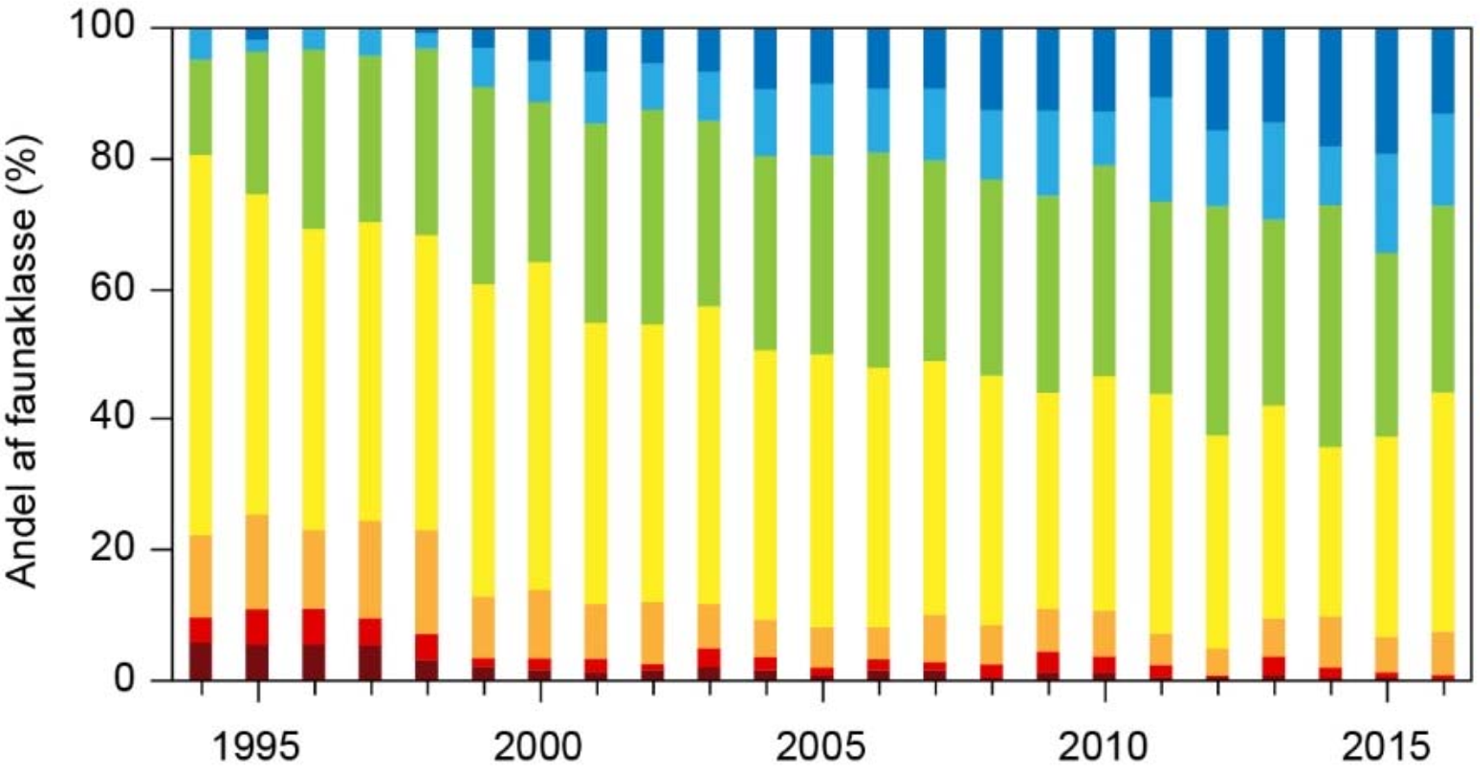
\includegraphics[width=\textwidth]{figures/DVFI}
\end{frame}

\begin{frame}{Søer $>$ 5 ha: Sommergennemsnit for klorofyl \textit{a}}
  \begin{itemize}
    \item 180 søer med faste kontroller.
    \item 447 søer med enkelte operationelle overvågninger.
  \end{itemize}
  \vfill
\end{frame}
\begin{frame}{Søer $>$ 5 ha: Sommergennemsnit for klorofyl \textit{a}}
  \begin{itemize}
    \item 180 søer med faste kontroller.
    \item 447 søer med enkelte operationelle overvågninger.
    \item Kerne af 29 søer med mange kontroller siden 1989:
  \end{itemize}
  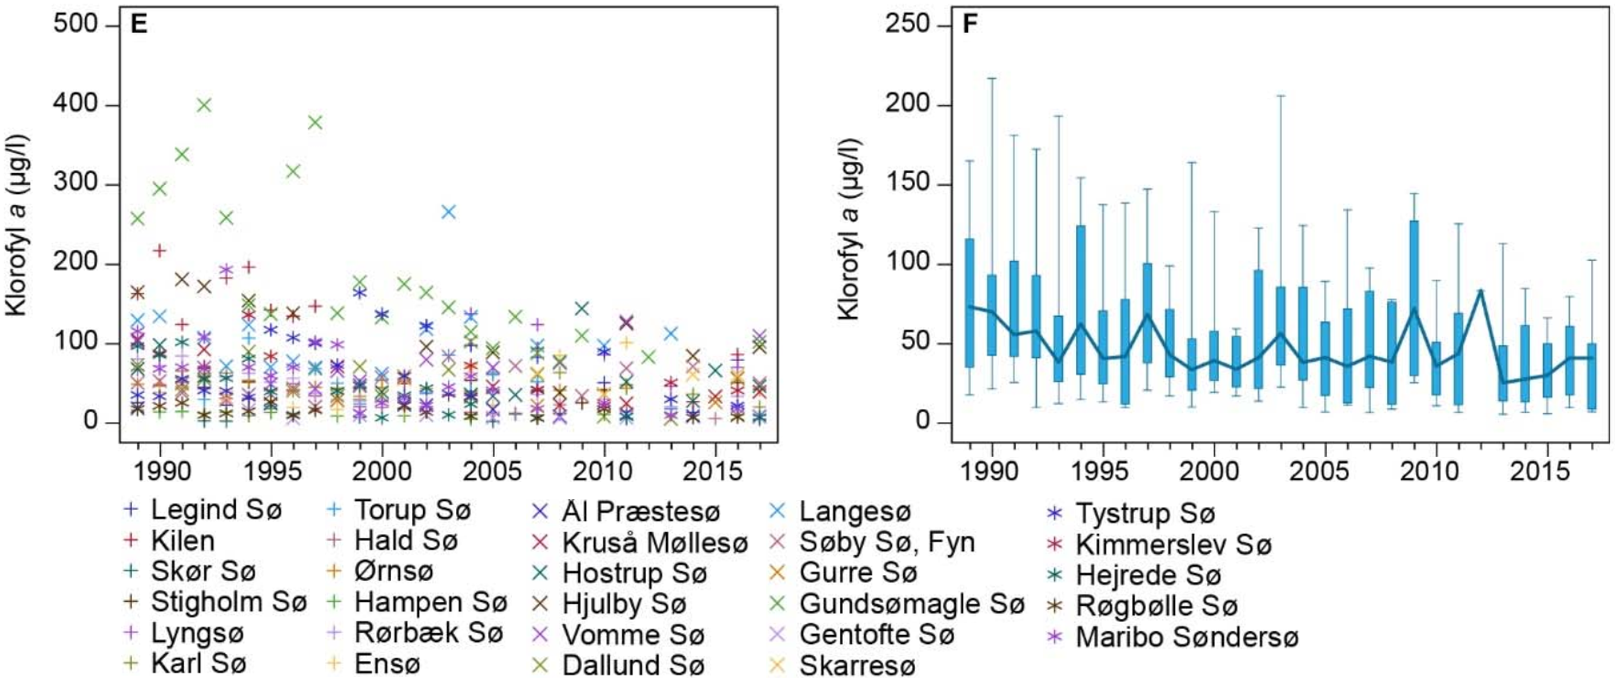
\includegraphics[width=\textwidth]{figures/chlorophyll_lakes}
\end{frame}

